% arara: pdflatex: { synctex: yes }
% arara: makeindex: { style: ctuthesis }
% arara: bibtex

% The class takes all the key=value arguments that \ctusetup does,
% and a couple more: draft and oneside
\documentclass[oneside]{ctuthesis}
\usepackage{siunitx}
\usepackage{nomencl}
\usepackage{setspace}
\usepackage{indentfirst}

%%%%%%%%%%%%%%%%%% insert images from other directory
\usepackage{graphicx}
\graphicspath{{./images/}}

%%%%%%%%%%%%%%%%%%%%%%%%%%%%%%%%%%%%%% this shit is here to break long url into more lines
\usepackage{url}
\makeatletter
\g@addto@macro{\UrlBreaks}{\UrlOrds}
%\makeatother



%%%%%%%%%%%%%%%%%%%%%%%%%%%%%%%%%%%%%% this shit is here to prevent breaking words on the edge of a line
\tolerance=1
\emergencystretch=\maxdimen
\hyphenpenalty=10000
\hbadness=10000


\ctusetup{
%	preprint = \ctuverlog,```%%%%%%%%%%%%%%%%%%%%%%%%% toto je cislo na kazde strance dole ktere tam nema byt
%	mainlanguage = english,
%	titlelanguage = english,
	mainlanguage = czech,
	otherlanguages = {czech},
	title-czech = {Low power wireless sensor network},
	title-english = {Low power wireless sensor network},
	subtitle-czech = {},
	subtitle-english = {},
	faculty = F3,
	department-czech = {Katedra telekomunikační techniky},
	department-english = {Department of Telecommunications Engineering},
	author = {Tomáš Hyhlík},
	supervisor = {Ing. Bc. Marek Neruda, Ph.D},
	supervisor-address = {},
	supervisor-specialist = {Ing. Bc. Lukáš Vojtěch, Ph.D},
	fieldofstudy-english = {Electronics and Communications},
	subfieldofstudy-english = {Electronics},
	fieldofstudy-czech = {Elektronika a komunikace},
	subfieldofstudy-czech = {Elektronika},
	keywords-czech = {sensor network},
	keywords-english = {sensor network},
	day = 12,
	month = 10,
	year = 2019,
	specification-file = {zav_prace.pdf},
%	front-specification = true,
%	front-list-of-figures = false,
%	front-list-of-tables = false,
%	monochrome = true,
%	layout-short = true,
}

\ctuprocess

\addto\ctucaptionsczech{%
	\def\supervisorname{Vedoucí}%
	\def\subfieldofstudyname{Studijní program}%
}

\ctutemplateset{maketitle twocolumn default}{
	\begin{twocolumnfrontmatterpage}
		% \ctutemplate{twocolumn.thanks}
		% \ctutemplate{twocolumn.declaration}
		\ctutemplate{twocolumn.abstract.in.titlelanguage}
		\ctutemplate{twocolumn.abstract.in.secondlanguage}	
		\ctutemplate{twocolumn.tableofcontents}
		\ctutemplate{twocolumn.listoffigures}
	\end{twocolumnfrontmatterpage}
}

% Theorem declarations, this is the reasonable default, anybody can do what they wish.
% If you prefer theorems in italics rather than slanted, use \theoremstyle{plainit}
\theoremstyle{plain}
\newtheorem{theorem}{Theorem}[chapter]
\newtheorem{corollary}[theorem]{Corollary}
\newtheorem{lemma}[theorem]{Lemma}
\newtheorem{proposition}[theorem]{Proposition}

\theoremstyle{definition}
\newtheorem{definition}[theorem]{Definition}
\newtheorem{example}[theorem]{Example}
\newtheorem{conjecture}[theorem]{Conjecture}

\theoremstyle{note}
\newtheorem*{remark*}{Remark}
\newtheorem{remark}[theorem]{Remark}

\setlength{\parskip}{5ex plus 0.2ex minus 0.2ex}

% Abstract in Czech
\begin{abstract-czech}
Účelem této práce je...

\end{abstract-czech}

% Abstract in English
\begin{abstract-english}
The purpose of this work is...
\end{abstract-english}

% % Acknowledgements / Podekovani
% \begin{thanks}
% I would like to thank Supervisor Ing. Bc. Marek Neruda Ph.D and Supervisor-specialist Ing. Bc. Lukáš Vojtěch Ph.D for helping me with this project. Also I would like to thank IMA s.r.o. company, which helped me to get compatible cards to the HID Prox Point plus reader, which is used for the second system design.
% \end{thanks}


% % Declaration / Prohlaseni
% \begin{declaration}
% I declare that I have developed the presented work independently and that I have
% listed all information sources used in accordance with the Methodical Guidelines on
% Maintaining Ethical Principles During the Preparation of Higher Education Theses.

% In Prague, \ctufield{day}.~\monthinlanguage{title}~\ctufield{year}
% \end{declaration}

% Only for testing purposes
\listfiles
\usepackage[pagewise]{lineno}
\usepackage{lipsum,blindtext}
\usepackage{mathrsfs} % provides \mathscr used in the ridiculous examples

\newcommand{\abbrlabel}[1]{\makebox[3cm][l]{\textbf{#1}\ \dotfill}}
\newenvironment{abbreviations}{\begin{list}{}{\renewcommand{\makelabel}{\abbrlabel}}}{\end{list}}


%%%%%%%%%%%%%%%%%%%%%%%%%%%%%%%%%  BEGIN %%%%%%%%%%%%%%%%%%%%%%%%%%%%%%%%%%%%%%%%%
\begin{document}

\maketitle

% \ctutemplate{specification.as.chapter}           % ZADANI BP

%\rule{\linewidth}{1pt}     % this shit was here for the url cut
\titlespacing*{\chapter}					{0pt}	{0ex}{0ex}
\titlespacing*{\section} 					{0pt}	{0ex}{-3ex}
\titlespacing*{\subsection} 			{0pt}	{0ex}{-3ex}
\titlespacing*{\subsubsection}		 {0pt}	{0ex}{-4ex}
\titlespacing*{\paragraph} 			{0pt}	{0ex}{-4ex}
\titlespacing*{\aubparagraph} 		{0pt}	{0ex}{-4ex}

\section{List of Abbreviations}
\begin{abbreviations}
	\item[BLE]   	Bluetooth Low Energy
	\item[I2C]   	Inter-integrated Circuit
	\item[IoT]		Internet of Things
	\item[IPv6] 	Internet Protocol version 6
	\item[ISM]		Industrial, scientific and medical

	\item[M2M]		machine to machine
	\item[RF]		Radio Frequency
	\item[RPMA]		Random Phase Multiple Access
	\item[SDK]	 	Software development kit
	\item[SF]		Spread factor
	\item[SPI]   	Serial Peripheral Interface 

\end{abbreviations}


% \chapter{Introduction}
This chapter presents background, purpose and objectives to make clear the goal of this thesis.


\section{Background}
RFID technology is happening to be very popular these days for various applications such as industrial automation, access control, animal identification, public transport, event ticketing, parking, electronic wallet, goods identification and many more.
The question is how secure this technology is. The answer is, that there are various manufacturers providing RFID (Radio Frequency Identification) devices with various security. Information delivered by the manufacturers about the security should be clear.


\section{Why electronic door lock?}
However, there are very secure door locks, commonly used mechanical door lock has a lot of disadvantages. It's easy to clone keys and it's even possible to open the door without the key. If a key is lost, changing the lock is needed, which could be even impossible in some cases. Somebody who finds the lost key would be able to open the door.
Electronic door lock  might came out with solutions of these problems, however every lock is possible to hack somehow. 
A key of electronic door lock is usually RFID tag or card, but it can be also mobile phone communicating via bluetooth interface etc.
The user's card may be also used in other applications, like electronic purse.
In case that user loses his card, the card can be deleted from the system.
There is also so many advantages like user info can be stored on the RFID card and part of the system might be a server where scanned cards are monitored. 


\section{Objectives}
The purpose of this thesis is to design and assembly an RFID based access control system composed of inexpensive RFID devices used today and examine its security and possibility of hacking it. 
In the conclusions, it's assessed if the information given by the manufacturer gives a clear picture of the security of
his RFID technology.















		

% \part{Theoretical part}
													
\chapter{Low power wireless network technologies}
todo prepsat do cj

\section{IQRF}
This technology aims to make it easy to implement wireless solutions. It enables peer-to-peer, star and mesh network communication modes. The IQRF alliance provide IQRF transceivers for \$15-20 with a few serial interfaces such as SPI, I2C, UART etc. and they also provide open source SDK which makes it very easy to use IQRF modules. The SDK is based on Java so it's compatible with various platforms such as Linux and Windows
\cite{1} \cite{2} \cite{3} \cite{4}.


\section{Wireless M-bus}
\textit{"Wireless Meter Bus has its origins within the Meter-Bus standards. This is a field bus standard aimed at applications for collecting meter data for gas, electricity, water, etc."} \cite{5}
It supports a few application modes for differing applications.
\begin{itemize}
  \item S1  Unidirectional, data are transmitted only a several times a day.
  \item S2	Bidirectional version of S1.
  \item	T1	Unidirectional transmission of data with a period of a few seconds of minutes.
  \item T2	Bidirectional version of T1.
  \item C1	Unidirectional transmission of bigger amount of data.
  \item C2	Bidirectional version of C1.
\end{itemize}
Usually one M-bus device support only a few of these application modes \cite{5} \cite{6} \cite{7} \cite{8}.


\section{Zigbee}
Zigbee, developed by zigbee alliance is usually used for mesh sensor networks because of its short range. This technology is standardized since 2003, so there is many available nodes at the market by now \cite{10} \cite{11} \cite{12}.

\section{Bluetooth}
Bluetooth has the big advantage, taht it's built in almost every mobile phone, tablet or laptop so there are more options to control the network. The Bluetooth 4.0+ also called BLE (Bluetooth Low Energy) aims to low power wireless sensor networks.
It can be used for point-to-point, broadcast or mesh network topology \cite{13} \cite{14} \cite{15} \cite{16}.


\section{LoRa}
The name LoRa stands for "Long Range" wireless communication with low data rate and power consumption. The protocol enables to modify SF which affects the communication range and data rate. The \ref{fig:loraSF} shows this dependence.

\begin{figure}[!h]
    \centering
    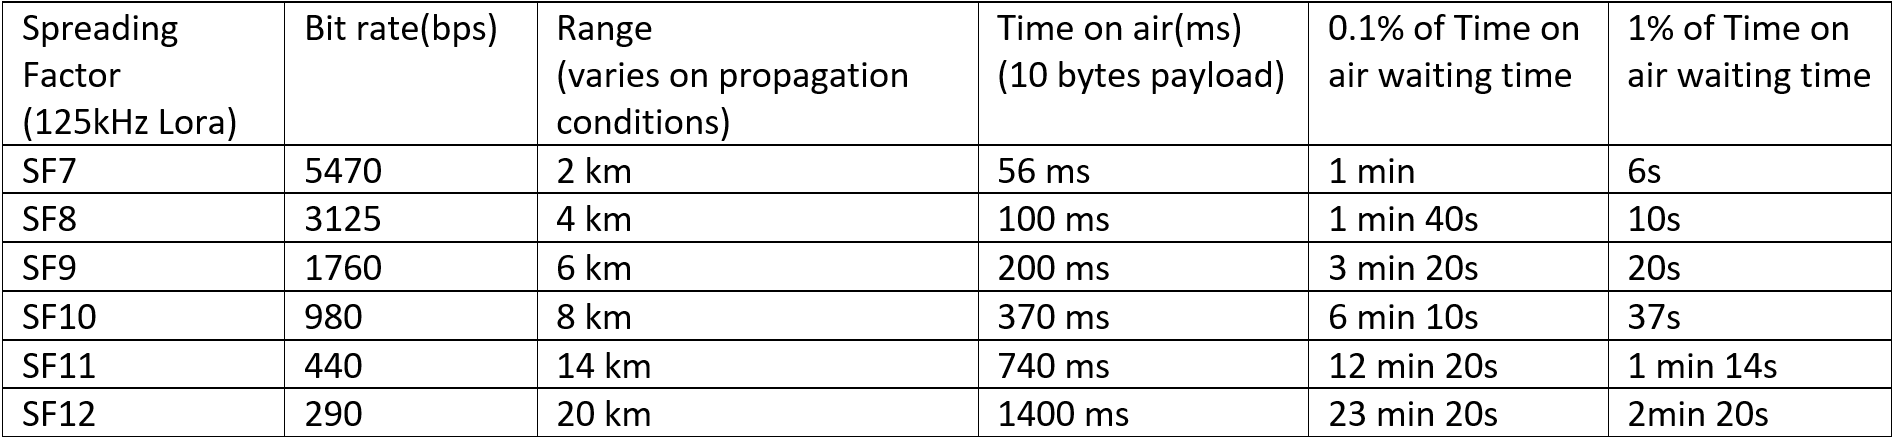
\includegraphics[width=1\textwidth]{spreading_factor_lorawan_2017-07-29}
    \caption{LoRa spread factor options \cite{24}}
    \label{fig:loraSF}
\end{figure}

This technology is very attractive for its long range capability and easy to connect nodes. It's complicated to build a full-capacity gateway which is capable of receiving packets at all frequency channels and SF in parallel. The transceiver for this application costs about \$130. Although it's also possible to build single-channel gateway which is way too cheaper, but it can receive packets at only one frequency channel and SF at once \cite{17} \cite{18} \cite{19} \cite{20} \cite{21} \cite{22} \cite{23} \cite{24}.


\section{Sigfox}
This technology focuses on short message and long range communication applications \cite{25} \cite{26}.


\section{Z-Wawe}
Z-Wave is intended for wireless connectivity for all possible smart home products, controlled by PC, phone, voice, etc. It's based on mesh network topology so every non-battery powered device works as a router to enhance the network range so the more devices are connected in one network, the stronger the network is \cite{27} \cite{28}.


\section{Thread}
This technology based on IPv6 was developed for home network controlled by smartphone, tablet or PC \cite{29} \cite{30} \cite{31}.


\section{RPMA}
The "Random Phase Multiple Access" developed by Ingenu designed for M2M and IoT applications \cite{32} \cite{rpma_ublox} \cite{34}. \textit{"RPMA has been deployed for the Machine Network, but can also be rolled out as a private network installation. It is highly suitable for regions, where the rollout of 3GPP LPWA technologies is lagging, where cellular coverage is generally weak, or where users would like to exert full control over their network deployments."}\cite{rpma_ublox}




\chapter{The design of the sensor network}
% This chapter describes the design of the sensor network.

\section{Block diagram}
\subsection{Node}
The node as an any device that transmits data in the network. In the star network topology it could be only a sensor or an actuator accessed by the gateway, because there are no routing devices or other. \cite{wsn01}.
\subsection{Gateway}
The gateway handles the communication with all the nodes and transmits the data to other network or device \cite{wsn01}. 
In this case the gateway is accessed by the LAN through RS-485 interface. 
\begin{figure}[!h]
    \centering
    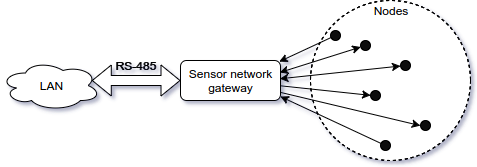
\includegraphics[width=1\textwidth]{LPwSN_bd}
    \caption{The block diagram of the sensor network}
    \label{fig:Typical structure of a card}
\end{figure}


\section{The requirements for the wireless technology}
The main requirement for the designed network is ability to add many various nodes which are available at the market to the network, so we don't have to make our own nodes for every kind of application.
The other requirements are price, power consumption, range etc.


\section{The final choose of the low power wireless technology}
From all the compared technologies in the table in appendix is chosen LoRa, because its nodes are easy to implement to the network with no restrictions. For example there is also many BLE nodes available at the market, but many of manufacturers say that their nodes are compatible only with their own network gateway so it may not be possible to add the node to our designed network. 
To make it simple and cheap only single channel gateway is used which means that all the devices in the network must be configured to one predefined channel and SF. 
															

% \part{Practical part}


\bibliographystyle{amsalpha}
% \bibliography{0main}	% not used
\bibliographystyle{csn690}
\bibliography{mybibliographyfile}
\begin{thebibliography}{9}
%%%%%%%%%%%%%%%%%%%%%%%%%%%%%%%%%%%%%%%%%%%%%%%%%%%%%%%%%%%%%%%



\bibitem[1]{nucleoST}
\textit{
NUCLEO-L073RZ.
}
ST Microelectronics
[Online]. Available:
\url{
https://www.st.com/en/evaluation-tools/nucleo-l073rz.html
}
[Accessed: 20-Sep-2019].

%___________________

\bibitem[2]{nucleoMbed}
\textit{
NUCLEO-L073RZ
}
ARM Mbed.
[Online]. Available:
\url{
https://os.mbed.com/platforms/ST-Nucleo-L073RZ/
}
[Accessed: 20-Sep-2019].

%___________________

\bibitem[3]{RFM95w}
\textit{
RFM95/96/97/98(W) - Low Power Long Range Transceiver Module}.
HopeRF electronic.
V1.0.
[Online]. Available:
\url{
http://wiki.dragino.com/index.php?title=Lora_Shield
}
[Accessed: 20-Sep-2019].

%___________________


\bibitem[4]{draginoWiki}
\textit{
Lora Shield.
}
Dragino.
[Online]. Available:
\url{
http://wiki.dragino.com/index.php?title=Lora_Shield
}
[Accessed: 20-Sep-2019].

%___________________


\bibitem[5]{AESlib}
\textit{
tiny-AES128-C
}
bitdust.
[Online]. Available:
\url{
https://github.com/bitdust/tiny-AES128-C
}
[Accessed: 20-Sep-2019].

%___________________


\bibitem[6]{CMAClib}
\textit{
openpana.
}
OpenPANA.
[Online]. Available:
\url{
https://github.com/OpenPANA/openpana
}
[Accessed: 20-Sep-2019].

%___________________


\bibitem[7]{rs485tr}
\textit{
SparkFun Transceiver Breakout - RS-485
}
Sparkfun.
[Online]. Available:
\url{
https://www.sparkfun.com/products/10124
}
[Accessed: 20-Sep-2019].


%___________________


\bibitem[8]{lwSpec}
\textit{
LoRaWAN Specification
}.
LoRa Alliance.
v1.1.
Sparkfun.
[Online]. Available:
\url{
https://lora-alliance.org/resource-hub/lorawantm-specification-v11
}
[Accessed: 20-Sep-2019].


%___________________


\bibitem[9]{lwSecur}
Robert Miller.
\textit{
LoRa Security
Building a Secure LoRa Solution.
}
MWR Labs Whitepaper.
[Online]. Available:
\url{
https://labs.mwrinfosecurity.com/assets/BlogFiles/mwri-LoRa-security-guide-1.2-2016-03-22.pdf
}
[Accessed: 20-Sep-2019].




% -------------------------
\bibitem[10]{accessControlSystem_eiprocus}
% \textit{

% }

[Online]. Available:
\url{
https://www.elprocus.com/understanding-about-types-of-access-control-systems/
}
[Accessed: 9-Sep-2019].


% -------------------------
\bibitem[11]{high density LPWAN}
% \textit{

% }

[Online]. Available:
\url{
https://ieeexplore.ieee.org/stamp/stamp.jsp?tp=&arnumber=8678997
}
[Accessed: 9-Sep-2019].

% -------------------------
\bibitem[12]{IoT cisco study}
% \textit{

% }

[Online]. Available:
\url{
https://blogs.cisco.com/innovation/the-internet-of-things-5-predictions-for-2018
}
[Accessed: 9-Sep-2019].

% % -------------------------
\bibitem[2]{IoT cisco study 02}
% \textit{

% }

[Online]. Available:
\url{
https://www.cisco.com/c/dam/en_us/about/ac79/docs/innov/IoT_IBSG_0411FINAL.pdf
}
[Accessed: 9-Sep-2019].

% % -------------------------
% \bibitem[2]{2}
% \textit{

% }

% [Online]. Available:
% \url{

% }
% [Accessed: 9-Sep-2019].

% % -------------------------
% \bibitem[2]{2}
% \textit{

% }

% [Online]. Available:
% \url{

% }
% [Accessed: 9-Sep-2019].

% % -------------------------
% \bibitem[2]{2}
% \textit{

% }

% [Online]. Available:
% \url{

% }
% [Accessed: 9-Sep-2019].

% % -------------------------
% \bibitem[2]{2}
% \textit{

% }

% [Online]. Available:
% \url{

% }
% [Accessed: 9-Sep-2019].





\end{thebibliography}


%\appendix



\end{document}